\documentclass{article}
\usepackage[utf8]{inputenc}  % Para caracteres acentuados
\usepackage{booktabs}        % Para \toprule, \midrule, \bottomrule
\usepackage{graphicx}        % Para inserir figuras
\usepackage{float}           % Para usar [H] e fixar posição da figura
\usepackage{lipsum}          % Para texto de exemplo (opcional)


\begin{document}
	
	% --- Gráfico centralizado template---
	\section*{Gráfico}
	
	
	\begin{figure}[H]
		\centering
		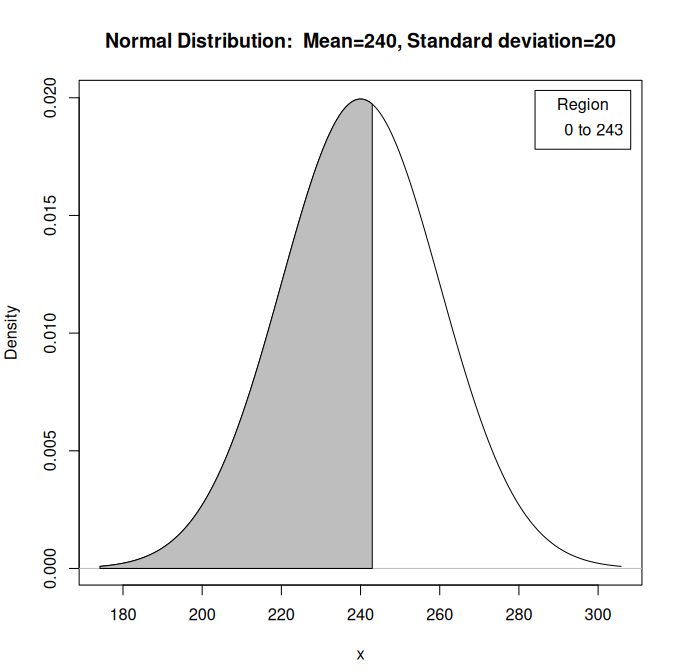
\includegraphics[width=0.7\textwidth]{/home/thallysson/AreaDeTrabalho/Semestre4_Disciplinas_Drive/Estatistica/latex/graficos/atv7_4a.png}
		% substitua pelo arquivo do seu gráfico
		\caption{Gráfico da distribuição normal de probabilidade das médias das amostras de 16 fracos de matéria prima para cosméticos com volume menor que 243ml}
		\label{fig:grafico_a}
	\end{figure}
	
	\begin{figure}[H]
		\centering
		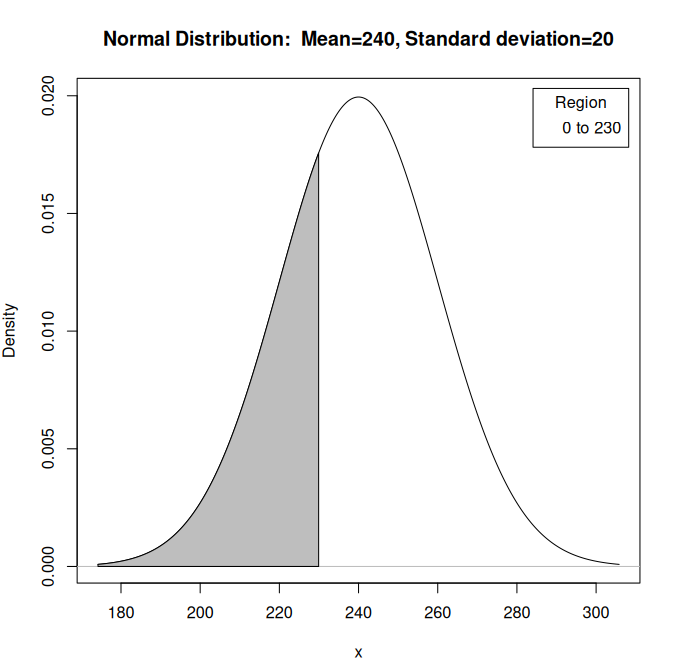
\includegraphics[width=0.7\textwidth]{/home/thallysson/AreaDeTrabalho/Semestre4_Disciplinas_Drive/Estatistica/latex/graficos/atv7_4b.png}
		% substitua pelo arquivo do seu gráfico
		\caption{Gráfico da distribuição normal de probabilidade das médias das amostras de 16 fracos de matéria prima para cosméticos com volume menor que 230ml}
		\label{fig:grafico_b}
	\end{figure}
	
	\begin{figure}[H]
		\centering
		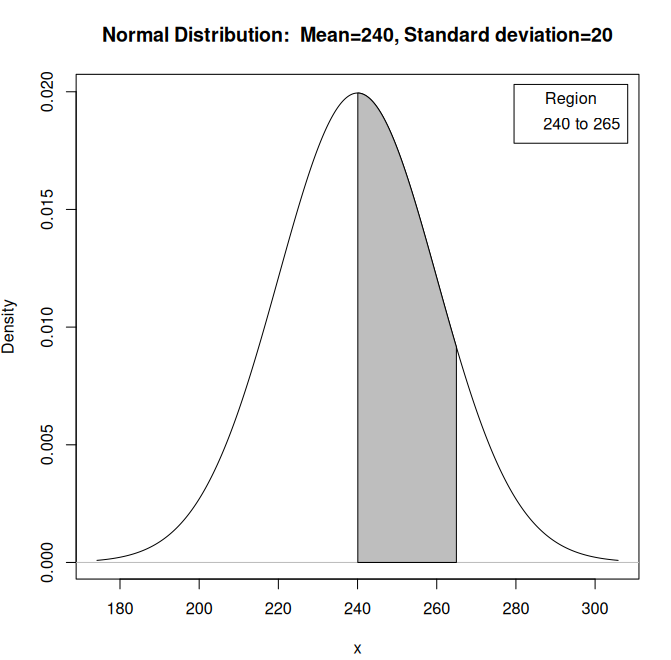
\includegraphics[width=0.7\textwidth]{/home/thallysson/AreaDeTrabalho/Semestre4_Disciplinas_Drive/Estatistica/latex/graficos/atv7_4c.png}
		% substitua pelo arquivo do seu gráfico
		\caption{Gráfico da distribuição normal de probabilidade das médias das amostras de 16 fracos de matéria prima para cosméticos com volume entre 240ml e 265ml}
		\label{fig:grafico_c}
	\end{figure}
	
	\begin{figure}[H]
		\centering
		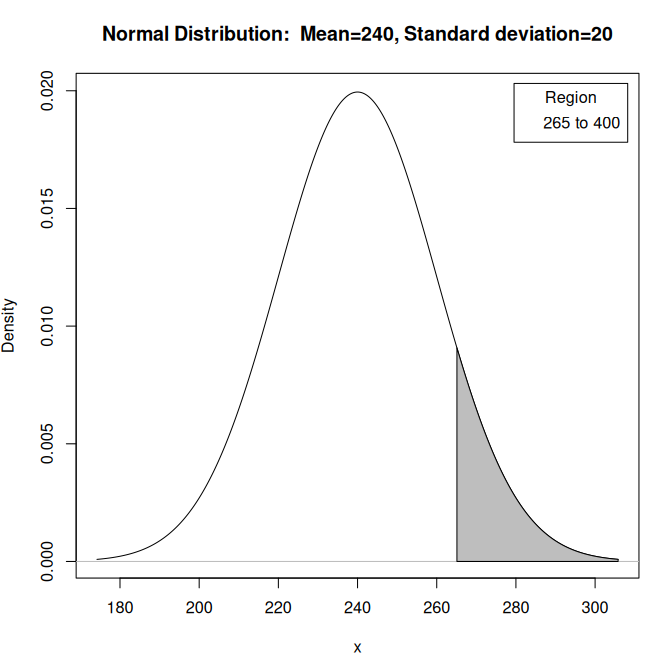
\includegraphics[width=0.7\textwidth]{/home/thallysson/AreaDeTrabalho/Semestre4_Disciplinas_Drive/Estatistica/latex/graficos/atv7_4d.png}
		% substitua pelo arquivo do seu gráfico
		\caption{Gráfico da distribuição normal de probabilidade das médias das amostras de 16 fracos de matéria prima para cosméticos com volume maior que 265ml}
		\label{fig:grafico_d}
	\end{figure}
	
	
	
	
	
\end{document}

